\section{Structure}

The class diagram is based on the classes and events, which was described earlier in chapter \ref{cap:classesevents}. The class diagram got a complex structure, after a person is registered in the helpdesk, the person is assigned to one or more roles. User and Staff inherit from role, because it is two different roles. A user can add problems to the helpdesk, a problem can be assigned to a staff member or a staff member can be assigned to a problem. A problem needs to be added to the helpdesk before a solution can exists. A problem can have no, one or more solutions assigned. Categories got a aggregation relationship to none, one or more tags, these tags can be assigned to problems. A department aggregates to staff and problem, a department can have none, one or more staffs and problems.  The class diagram is illustrated at figure \ref{fig:pdaclassdiagram}

\begin{figure}
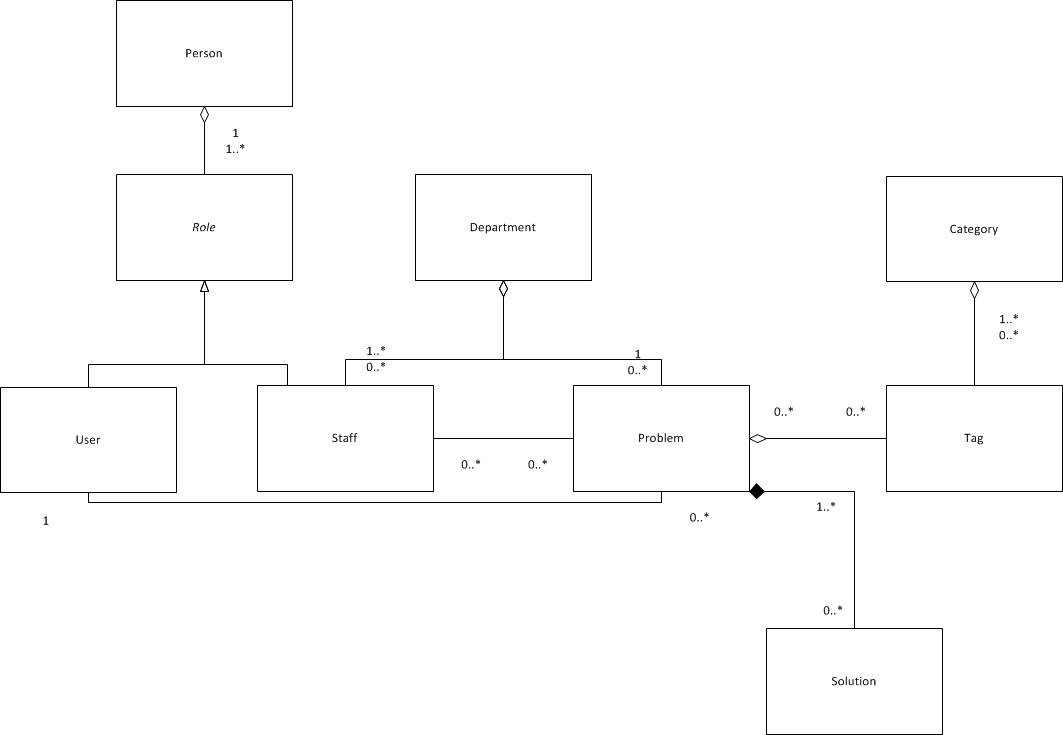
\includegraphics[width=100pt]{input/problem_domain_analysis/Klasse_diagram.jpg}
\caption{hej}
\label{fig:pdaclassdiagram}
\end{figure}